 \documentclass[10pt,oneside,swedish]{lips-no_customer}

%\usepackage[square]{natbib}\bibliographystyle{plainnat}\setcitestyle{numbers}
\usepackage[yyyymmdd]{datetime}
\renewcommand{\dateseparator}{-}
\usepackage[round]{natbib}\bibliographystyle{plainnat}
\usepackage{parskip}
%\usepackage{subfigure}
%\usetikzlibrary{decorations.pathreplacing,angles,quotes}

\usepackage{pgfplots}
\usepackage{pgfplotstable}

% Configure the document
\title{Teknisk dokumentation}
\author{Yc4}
\date{\today}
\version{1.1}

\reviewed{Erik Frisk och Britta Önnegren}{2019-12-06}
\approved{}{}

\projecttitle{Styrning och optimering av bilbana}

\groupname{Yc4}
\groupemail{team\_yc4@liuonline.onmicrosoft.com}
\groupwww{https://www.fs.isy.liu.se/Edu/Courses/TFYY51/}

\coursecode{TFYY51}
\coursename{Ingenjörsprojekt}

\orderer{Erik Frisk, Linköpings universitet}
\ordererphone{+46(0)13-285714}
\ordereremail{erik.frisk@liu.se}

%\customer{Kund, Företag X}
%\customerphone{+46 xxxxxx}
%\customeremail{erik.frisk@liu.se}

\courseresponsible{Urban Forsberg}
\courseresponsiblephone{+46(0)13-281350}
\courseresponsibleemail{urban.forsberg@liu.se}

\supervisor{Viktor Leek}
\supervisorphone{+46(0)13-284493}
\supervisoremail{viktor.leek@liu.se}

\smalllogo{logo} % Page header logo, filename
\biglogo{logo} % Front page logo, filename

\cfoot{\thepage}
\begin{document}
\maketitle

\cleardoublepage
\makeprojectid

\begin{center}
  \Large Projektdeltagare
\end{center}
\begin{center}
  \begin{tabular}{|l|l|l|} \hline
    \textbf{Namn} & \textbf{Ansvar} & \textbf{Kontaktinformation }\\\hline

    Mattias Uvesten & Projektledare (PL) & 0768697559\\
    && \url{matvu053@student.liu.se} \\\hline

    Gustav Sörnäs & Dokument, display (DOK, DSP) & 0703279113\\
    && \url{gusso230@student.liu.se} \\\hline

    Alexander Tuneskog & Hastighet (SPD) & 0725559873 \\
    && \url{aletu130@student.liu.se} \\\hline

    David Thorén & Tester, gemensam målgång (TST, GML) & 0721838605 \\
    && \url{davth346@student.liu.se} \\\hline

    Albin Wahlén & Kalibrering, positionering (KLB, POS) & 0762016054 \\
    && \url{albwa833@student.liu.se} \\\hline
  \end{tabular}
\end{center}

\section*{Dokumenthistorik}
\begin{tabular}{|p{.06\textwidth}|p{.1\textwidth}|p{.45\textwidth}|p{.13\textwidth}|p{.13\textwidth}|} 
  \hline
  \multicolumn{1}{|c}{\bfseries Version} &
  \multicolumn{1}{|c}{\bfseries Datum} &
  \multicolumn{1}{|c}{\bfseries Utförda förändringar} &
  \multicolumn{1}{|c}{\bfseries Utförda av} &
  \multicolumn{1}{|c|}{\bfseries Granskad}\\
  \hline\hline
  0.1 & 2019-11-28 & Struktur & Alla & \\\hline
  0.2 & 2019-11-30 & Första utkast & Alla & \\\hline
  0.3 & 2019-12-01 & Andra utkast & Alla & 2019-12-02 \\\hline
  0.4 & 2019-12-02 & Tredje utkast & Alla & \\\hline
  1.0 & 2019-12-03 & Färdig version & Alla & 2019-12-06 \\\hline
  1.1 & 2019-12-12 & Kommentarer från EF och språklärare & Alla & \\\hline

\end{tabular}

\cleardoublepage
\pagenumbering{arabic}\cfoot{\thepage}
% \section*{Sammanfattning}
Massa text som sammanfattar hela skiten.



\cleardoublepage
\tableofcontents
\cleardoublepage

\section{Inledning}

\subsection{Bakgrund} Projektet har utförts med hjälp av en bilbana samt
flera bilar, givare, spänningsaggregat och två datorer inne i bilbanerummet. Via datorn har spänning tillförts till bilbanan. Med hjälp av givarna är
det möjligt att veta när en bil har passerat en givare.  Programvaran har utvecklats
i Matlab.

\subsection{Syfte och mål}

Syftet med projektet är att lära sig att arbeta i projekt utifrån projektmodellen Lips. Målet med projektet är att konstruera ett system som klarar av alla krav som finns i kravspecifikationen. Se kravspecifikationen \ref{app:kravbeskrivning} samt kursmål.
\section{Begrepp och systemöversikt}

\section{Systembeskrivning}

% Systemet funktion vid starten är att öka oftare i början bootstrapen
% (exempelvis innan målgivaren) för att sedan öka mindre frekvent i segment 1.
% Bootsrapen (uppstarten) avslutas efter segment 3. 

\begin{figure}
	\centering
	\includegraphics [height=0.8\textheight] {Figures/flow}
	\caption{Flödesschema över systemet.}
	\label{fig:flow}
\end{figure}

Systemet är indelat i olika delsystem efter huvudsaklig funktionalitet enligt figur
\ref{fig:flow}. Nedan beskrivs dessa delsystem i mer detalj.

\subsection{Innan start}

Vid uppstart ritas knappar ut på displayen, se figur \ref{fig:choose1} och \ref{fig:choose2}. Med dessa knappar går
det att välja om en eller två banor ska vara aktiva och om de ska styras
autonomt av systemet eller manuellt med handkontroll. Det går också att ställa
in en referenstid mellan 12 och 15 sekunder med 0,5 sekunders intervall genom
att trycka på + och - på displayen. 
\begin{figure}
	\centering
	\includegraphics[width=\linewidth] {Figures/choose1}
	\caption{Display före start}
	\label{fig:choose2}
\end{figure}
\begin{figure}
	\centering
	\includegraphics [width=\linewidth] {Figures/choose2}
	\caption{Display före start}
	\label{fig:choose2}
\end{figure}

\subsection{Uppstart} 
\label{sec:systembeskrivning:uppstart}
Vid autonom körning utgår systemet ifrån en bootstrap som är systemet för uppstarten av bilarna. Då körs funktionen \texttt{do\_boot()} som arbetar fram en
initial \texttt{car.constant}. Detta sker i tre steg. Innan bilen börjar rulla
höjs \texttt{car.constant} varje 0,7 sekunder. När bilen börjar rulla och åker
under målgivaren höjs \texttt{car.constant} långsammare tills bilen åkt under
den första givaren varpå \texttt{car.constant} inte längre ändras. Vid den
tredje givaren jämförs hur lång tid det senaste segmentet tog att köra och en
sista \texttt{car.constant} räknas ut som förväntas ge en varvtid på 15
sekunder. Om den förväntade varvtiden är längre än 15 sekunder höjs
\texttt{car.constant} och om den förväntade varvtiden är lägre sänks
\texttt{car.constant}.

\begin{figure}
	\centering
	\begin{tikzpicture}
		\draw 
			(0,0) -- 
			(1,0) --
			(1,1) --
			(2,1) --
			(2,2) --
			(3,2) --
			(3,3) --
			(4,3) --
			(4,5) --
			(7,5) --
			(7,5.5) --
			(10,5.5);
		\draw [dotted] (10, 5.5) -- (14, 5.5);
		\draw [->] (0,0) -- (15, 0) node[right]{$t$};
		\draw [->] (0,0) -- (0, 8) node[above]{Spänning};
		\draw [dotted] (4, 0) -- (4, 0.5) node[right]{Målgivarutslag} -- (4,3);
		\draw [dotted] (10,0) -- (10, 3) node[right]{Bootstrap slut} -- (10, 5.5);
		\draw [decoration={brace, raise=2pt}, decorate] (1,1) -- (2,1);  % dt
		\node at (1.5, 1.5) {$dt_1$};
		\draw [decoration={brace, raise=2pt}, decorate] (1,0) -- (1,1);
		\node at (0.5, 0.5) {$dU_1$};
		\draw [decoration={brace, raise=2pt}, decorate] (4,3) -- (4,5);
		\node at (3.5, 4) {$dU_2$};
		\draw [decoration={brace, raise=2pt}, decorate] (4,5) -- (7,5);
		\node at (5.5, 5.5) {$dt_2$};
		\draw [decoration={brace, mirror, raise=2pt}, decorate] (7,5) -- (7,5.5);
		\node at (7.55,5.25) {$dU_3$};
	\end{tikzpicture}
	\caption{Metod för start av bil.}
	\label{fig:bootstrap}
\end{figure}

\subsection{Körning}
\label{sec:systembeskrivning:korning}

Huvudloopen körs åtminstonde 10 gånger i sekunden. Den beräknar var bilen
befinner sig, hur snabbt bilen ska köra och skickar det nya gaspådraget till
banan. När en givare passeras justeras också bilens konstant efter nuvarande
varv- och referenstid. Nedan beskrivs vad systemet gör under en komplett
programcykel.

\subsubsection{Position}
\label{sec:system:korning:position}

Om en givare passerats vet systemet exakt var bilen befinner sig. Om så är
fallet sparas den nuvarande exakta position och kallas \emph{givarpositionen}.

% Om en ny givare har passerats, \texttt{car.new\_check\_point == true}, ökar
% programmet nuvarande segment (\texttt{car.segment}) med 1. \texttt{car.segment}, som
% alltid ligger mellan 1 och 9, används som index för att välja position i en
% lista (\texttt{car.pos\_at}). Vi kallar den positionen för \emph{givarpositionen}.

Oavsett om en givare passerats eller inte räknar systemet ut en beräknad
position. Detta görs genom att räkna ut en approximativ hastighet $v =
\frac{s}{t}$ där $v$ är hastigheten, $s$ är längden på det nuvarande segmentet
och $t$ är hur lång tid det nuvarande segmentet tog förra varvet.

% Om ingen givare har passerars och första varvet är avslutat kallas först på funktionen \texttt{get\_approx\_v()}. Denna utgår ifrån
% förra varvets segmentstider (\texttt{car.seg\_times}) och segmentslängder
% (\texttt{car.seg\_len}) och beräknar med $v = \frac{s}{t}$, där \texttt{s} är segmentslängden och \texttt{t} segmentstiden, \texttt{v} som är medelhastigheten för nuvarnade
% segment, men förra varvet. Denna antas vara ungefär samma som nuvarande
% hastiget och kallas \emph{car.v}. 

Med den approximativa hastigheten räknas sedan en beräknad längd bilen rört sig
sedan senaste programcykeln ut med $\mathrm{d}s = v \cdot \mathrm{d}t$ där
$\mathrm{d}s$ är den beräknade sträckan bilen rört sig, $v$ är hastigheten som
precis räknades ut och $\mathrm{d}t$ är tiden sedan den förra programcykeln.
Denna förflyttning adderas med positionen från förra programcykeln och kallas
den \emph{beräknade positionen}.

Om en givare passerats räknar systemet här ut om en givare vid ett tidigare
tillfälle passerats (genom att jämföra givarpositionen och den beräknade
positionen). Information om denna procedur finns i del~\ref{sec:missade givare}.

% Sedan beräknas positionen, i meter från målgivaren, med funktionen
% \texttt{get\_position()}. Den använder den ungefärliga hastigheten \texttt{v} beräknad av
% \texttt{approx\_v()} och tiden \texttt{t} sedan denna beräkning gjordes senast (en programcykel, se \ref{sec:system:korning:cykel})
% och beräknar med $s = v \cdot t$ den sträcka som bilen har åkt. Sedan adderas denna
% med förra kända positionen och returneras i \texttt{car.position}. Denna 
% \emph{beräknade} position tas också fram när en givare har passerats, då skrivs den över med \emph{givarpositionen} men används i stället för att detektera missade givare. Se \ref{sec:missade givare}.

\subsubsection{Gaspådrag}

Efter positionsberäkningen beräknas spänningen som ska skickas till banan. Detta
görs genom att multiplicera det önskade spänningsvärdet för den nuvarande
positionen från kartan med bilens konstant.

% Efter positionsberäkningen beräknas det gaspådrag som skall sättas till banan. Detta görs i två
% funktioner, \texttt{get\_new\_v} och \texttt{get\_new\_u}.
% 
% I \texttt{get\_new\_v} används bilens nuvarande postition (\texttt{car.postition})
% och hastighetskartan (\texttt{car.map}). I \texttt{car.map} finns en
% hastighetsparameter för varje \texttt{car.position} (Se \ref{sec:begrepp och systemöversikt}.), denna retuneras av funktionen
% och sparas i \texttt{car.v}.
%  
% I \texttt{get\_new\_u} används denna hastighetsparameter tillsammans med
% \texttt{car.constant}. Dessa multipliceras och deras produkt retuneras och sparas
% i \texttt{car.u}.

\subsubsection{Governor}
\label{sec:systembeskrivning:governor}

Om bootstrap är avslutad och en givare passerats behöver bilens konstant
eventuellt justeras. 

För att justera bilens konstant behöver systemet först beräkna hur lång tid det
nuvarande varvet kommer ta. Vid varje givare beräknas därför den genomsnittliga
hastigheten genom det förra segmentet och multipliceras med den kvarvarande
sträckan på varvet för att få den uppskattade tiden den resterande delen av
varvet kommer ta. Denna tid läggs ihop med varvtiden hittils och ger då en
uppskattad varvtid för det nuvarande varvet. Denna varvtid jämförs sedan med den
valda referenstiden och bilens konstant anpassas vid behov.

% Detta görs med funktionen \texttt{do\_gov}.  Först görs en uppskattning av 
% varvtiden utifrån hur lång tid varvet har tagit än
% så länge. Detta görs med forecasts som beräknar den approximerade varvtiden utifrån tid fram tills senast
% passerad givare samt hastighet i tidigare segment. Genom att veta en
% genomsnittlig hastighet går det med kvarvarande sträcka att räkna ut en
% ungefärlig kvarvarande tid. När tiden från mål till senaste passerade givare adderas med
% den uträknade approximerade tiden kvar, så erhålls det en uppskattad varvtid som
% används för att avgöra om en bil behöver åka snabbare eller långsammare. Om bilen dock är inne på sitt första varv görs uppskattningen endast
% utifrån förra segmentet \texttt{car.forcasts\_naive} och om första varvet är
% avslutat så används \texttt{car.forcasts} som vanligt. Detta görs efter segment 4 och 8. Dessutom används den
% faktiska varvtiden när bilen passerar mål (från varv 2 och frammåt).
%  
% Sedan jämförs denna uppskattade varvtid med referenstiden (\texttt{car.ref\_time}) 
% och \texttt{car.constant} justeras.

% \begin{verbatim}
% car.constant = car.constant + (status - 1) * 0.08;
% \end{verbatim}

% Där \texttt{status} är den uppskattade varvtidens förhållande till \texttt{car.ref\_time}.
% D.v.s om de är exakt lika blir \texttt{status~ =~ 1}, om uppskattningen är högre blir
% den större än 1 och om den är lägre blir den mindre än 1. Således kommer \texttt{car.constant}
% höjas eller sänkas proportionellt mot hur långt ifrån \texttt{car.ref\_time} uppskattningen
% av varvtiden ligger. 

\subsubsection{Hantering av längden av en programcykel}
\label{sec:system:korning:cykel}

I slutet av varje cykel körs en loop som tillfälligt pausar programmet.
För att få avläsningen att ske minst en gång var tionde sekund pausas
programmet kontinuerligt 0,001 sekunder tills den totala paustiden överskrider 
0,07 sekunder då nästa cykel börjar. Då pausen på 0,001 sekunder är så pass
kort och marginalen till kravet är rätt stor så sker avläsningen mellan
0,07 och 0,1 sekunder. Längden på den största skillnaden mellan två avläsningar
sparas och visas vid programmets slut.


\subsubsection{Display}

I varje programcykel skickas värdet på \texttt{car.u} till två stapeldiagram på
displayen för vardera bil. Se \ref{app:funktioner och filer:display} för information om displayens
stapeldiagram. Om ett nytt varv inleds skrivs dessutom förra varvnumret och
varvtiden ut på displayen.


\subsection{Avslut}

För att avbryta programmet manuellt kan användaren när som helst trycka på q
eller s på datorns tangentbord. Trycker användaren på q avslutas programmet
direkt. Trycker användaren på s stoppas varje bil var för sig och fordonet
stoppas när programmet uppskattar att bilen befinner sig 80~cm innan målgivaren.
Därefter avslutas programmet när båda bilarna stannat.

Om det har gått mer än nio sekunder sedan en givare passerades pausas programmet
och användaren informeras på styrdatorn att en bil misstänkts ha fastnat eller
åkt av banan. 

När körningen avslutas slutar systemet skicka spänning till banan.
Om en bil kört fler än två varv sparas statistik från körningen i en
\texttt{.mat}-fil med nuvarande datum och tid som filnamn.

Vid programslut visas statistik om varvtid och genomsnittlig segmenttid på
displayen. Se figurer xx-xx.


\section{Händelser}

\subsection{Avslutning av körning}

För att avbryta programmet manuellt kan användaren när som helst trycka på s
eller q på datorns tangentbord. Trycker användaren på q avslutas programmet
direkt. Trycker användaren på s stoppas varje bil var för sig när de är 80~cm
från målgivaren och programmet avslutas när båda bilarna står stilla.

Om det har gått mer än nio sekunder sedan en givare passerades pausas programmet
och användaren informeras på styrdatorn att en bil misstänkts ha fastnat eller
åkt av banan. 

Vid programslut visas statistik om varvtid och genomsnittlig segmenttid på
displayen. Se figurer xx-xx.

\subsection{Missade givare}

Programmet gör redan en uppskattning av bilens position (\emph{get\_position})
 och justerar denna vid ny givare (lägg till referens här).
Eftersom \emph{get\_new\_v} utgår ifrån denna uppskattning, kommer ingen
anpassning behöva göras ifall en givare inte ger utslag. Däremot måste det 
kompenseras nästa gång en givare detekteras. Detta görs med funktionen 
\emph{choose\_position}. Den funktionen jämför positionen beräknad av 
\emph{get\_position} och positionen vald av nuvarande givare. 

Vid varje givare kollar \emph{choose\_position} vilken givare som 
\emph{get\_position} ligger närmast. Funktionen beräknar skillnaden mellan denna
och den givare som valdes med givardetektionen. Denna kallas \emph{seg\_plus}.
I normala fall är \emph{seg\_plus} = 0 (ingen 
missad givare) eller 1 (en missad givare), men den kan också bli högre. Eftersom
programmet inte ska behöva hantera för många givarsignaler ska \emph{seg\_plus}
aldrig kunna bli lägre än 0. Om så ändå är fallet ändras denna till 0. \emph{seg\_plus} 
retuneras av funktionen och används sedan för att höja \emph{car.segment} så att
programmet har koll på var bilen är.

Dessutom behöver den insamlade datan justeras när en eller flera givare har 
missats. Annars kommer \emph{car.seg\_times} spara tiden för flera segment som 
om det vore ett enda. Lösningen är att skriva över denna tid med 0. Alla 
funktioner som använder denna data behöver kolla ifall den är noll eller inte, 
om den är noll används den ifrån varvet innan i stället. Om den också är noll 
används den från två varv tidigare osv.

\section{Programslut}

display\_post\_race\_graphs(seg\_times1, seg\_times2, lap\_times1, lap\_times2,
ref\_time) hanterar knapptryck för att byta mellan de två vyerna. Varje 0,4
sekunder skickas ett kommando till displayen som kopierar det interna minnet
till minnet som delas med styrdatorn. Minnet som delas med styrdatorn läses av
och eventuella knapptryck hanteras genom anrop till antingen
draw\_lap\_graph(...) eller draw\_segment\_graph(...).

draw\_lap\_graph(lap\_times1, lap\_times2, ref\_time) ritar varvtider för
ena bilen i taget och skriver ut medelvärde och standardavvikelse, se figur xx.

Hur mycket ska jag skriva om implementationen här?

draw\_segment\_graph(seg\_times1, seg\_times2)

Samma fråga här som raden ovanför.

\section{Resultat}

Vid redovisningstillfället slutfördes två körningar på 15 varv vardera där de
fem första var kalibreringsvarv (enligt krav 20 och 22). Vid den första
körningen var referenstiden inställd på 13 sekunder och vid den andra var
referenstiden inställd på 14 sekunder. De två körningarna finns uppritade i
figur~\ref{fig:laptimes-calibration} med kalibreringsvarven och i figur~
\ref{fig:laptimes-no-calibration} utan kalibreringsvarven med vald referenstid
och den maximalt tillåtna avvikelsen på 0,5 sekunder (enligt krav 21) inritat.
Figur~\ref{fig:segtimes} visar den genomsnittliga segmentstiden vid vardera
körning.

Vid den första körningen höll bilen en genomsnittlig varvtid på 13,22~sekunder
med en standardavvikelse på 0,24~sekunder. $\pm$0,5~sekunder överträddes vid två
av varven med varvtider på 13,54 och 13,52~sekunder.

Vid den andra körningen höll bilen en genomsnittlig varvtid på 14,47~sekunder
med en standardavvikelse på 0,26~sekunder. $\pm$0,5~sekunder överträddes vid
fyra av varven med en maximal överträdelse på 0,31~sekunder långsammare än
maximal tillåten varvtid (14,5~sekunder).

Ingen av dessa körningar uppfyllde kraven på prestanda, alltså krav 20, 21 och
23.

Givarna lästes av mer än 10 gånger per sekund. Se \ref{sec:system:korning:cykel} för information om hur
detta mäts.

\begin{figure}
	\centering
	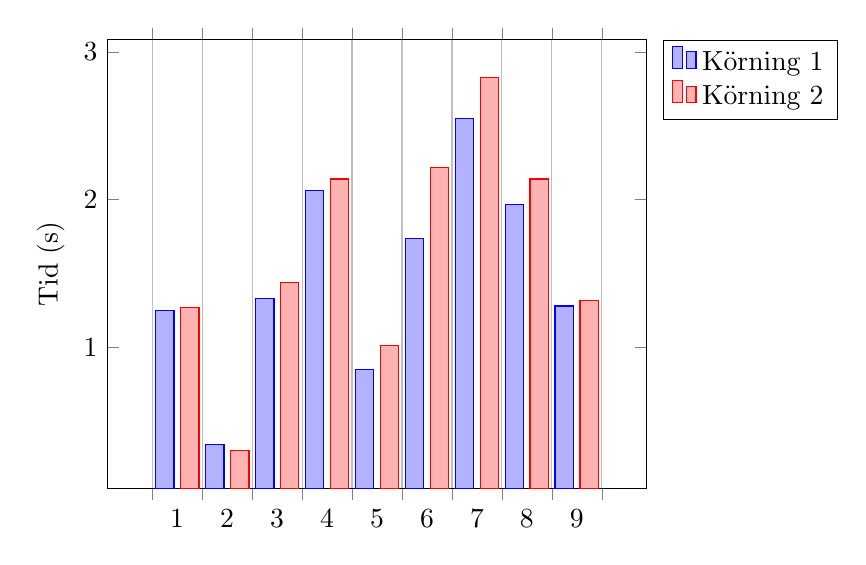
\begin{tikzpicture}
		\begin{axis} [
				ylabel=Tid (s),
				legend pos = outer north east,
				ybar interval=0.75
		]
			\addplot+ [] coordinates {(1, 1.25) (2, 0.34) (3, 1.33) (4, 2.06) (5, 0.85)
			(6, 1.74) (7, 2.55) (8, 1.97) (9, 1.28) (10, 1)};
			\addlegendentry{Körning 1}
			\addplot+ [] coordinates {(1, 1.27) (2, 0.30) (3, 1.44) (4, 2.14) (5, 1.01)
			(6, 2.22) (7, 2.83) (8, 2.14) (9, 1.32) (10, 1)};
			\addlegendentry{Körning 2}
		\end{axis}
	\end{tikzpicture}
	\caption{Genomsnittlig segmentstid för de två körningarna från redovisningen.}
	\label{fig:segtimes}
\end{figure}

\begin{figure}
	\centering
	\begin{tikzpicture}
		\begin{axis} [xmin=0, xmax=15.5,ymin=10,ymax=20, xlabel=Varv, ylabel={Tid (s)}, 
						legend pos=outer north east]
			\addplot+ [blue, mark options={blue}, mark=square*] table [col sep=comma, x index=0, y index = 1] {stats/lap.csv};
			\addlegendentry{Körning 1}
			\addplot+ [red, mark options={red}, mark=*] table [col sep=comma, x index=0, y index = 2] {stats/lap.csv};
			\addlegendentry{Körning 2}
		\end{axis}
	\end{tikzpicture}
  \caption{Varvtider för de två körningarna från redovisningen, inklusive
	kalibreringsvarven.}
	\label{fig:laptimes-calibration}

	\vspace*{\floatsep}% https://tex.stackexchange.com/q/26521/5764

	\begin{tikzpicture}
		\begin{axis} [xmin=5.5, xmax=15.5,ymin=12,ymax=16, xlabel=Varv, ylabel={Tid (s)}, 
						legend pos=outer north east]
			\addplot+ [blue, mark options={blue}, mark=square*] table [col sep=comma, x index=0, y index = 1] {stats/lap.csv};
			\addlegendentry{Körning 1}
			\addplot[blue, domain=0:20] {13};
			\addlegendentry{Referenstid körning 1}
			\addplot+ [red, mark options={red}, mark=*] table [col sep=comma, x index=0, y index = 2] {stats/lap.csv};
			\addlegendentry{Körning 2}
			\addplot [red, domain=0:20] {14};
			\addlegendentry{Referenstid körning 2}
			\draw[dotted] (axis cs:0,12.5) -- (axis cs:16,12.5);
			\draw[dotted] (axis cs:0,13.5) -- (axis cs:16,13.5);
			\draw[dotted] (axis cs:0,14.5) -- (axis cs:16,14.5);
		\end{axis}
	\end{tikzpicture}
	\caption{Varvtider för de två körningarna från redovisningen, exklusive
	kalibreringsvarven.}
	\label{fig:laptimes-no-calibration}
\end{figure}


\cleardoublepage
\appendix
\section{Handhavande}
Starta Matlab 2015b. Observera att användaren måste använda datorn som finns
inne i bilbanerummet och som är inkopplade till bilbanan. Inne i Matlab ska användaren navigera sig till yc4 mappen och öppna den. Därefter markera och högerklicka på mappen kod och välj alternativet ''Add To Path''. Klicka på ''Select Folders And Subfolders'' som dyker upp när musen pekar på ''Add To Path''. Därefter expandera bilbana mappen följt av yc4 mappen. Öppna sedan main.m och starta systemet genom att klicka på Run i Editorn i Matlab.

Därefter välj vilka banor som ska köras via den externa touch displayen. Justera också referenstiden genom att klicka på plusstecknet eller minustecknet (notera att referenstiden ändras med 0.5 s intervall). Kryssa även i om någon av banorna ska köras manuellt. Starta genom att trycka på knappen nere i det högra hörnet på displayen. Observera att bilarna måste placeras några decimeter innan målgivaren före start.

När programmet ska avslutas klickar användaren i kommentar fönstret i Matlab och
klickar på q om bilen ska stanna direkt. Om användaren istället vill att
bilen/bilarna ska stanna precis innan målgivaren klickar användaren på s
(observera att detta fungerar endast efter varv ett).

När programmet avslutas finns möjligheterna att se varvtiden/varvtiderna,
segmentstiden/segmentstiderna samt att avsluta. Detta väljs utifrån de tre
knapparna längst ner på displayen. Dessa knappar är Varv för att se varvtid,
Segment för att se segmentstider. Samt knappen Avsluta.

Om knappen Varv väljs kommer information såsom ''target'' vilket är vald varvtid.
“mean” som är genomsnittlig varvtid och “Stdev” är standardavvikelsen. För att
se varvtiden för den andra banan klicka på knappen uppe i högra hörnet.

Om programmet kraschar: Om programmet kraschar öppna main.m. Därefter skriv in
ctrl och enter i avgränsningen som heter ''\%\% END OF RACE'' som finns i slutet av
koden main.m.

\section{Funktioner och filer}

\subsection{System}

choose\_position(position, segment, track, track\_len)

Körs när en givare passerats. Gör en bedömning om en givare (eller flera) har
missats genom att kontrollera vilken givare som är närmast den nuvarande
uppskattade position och kompenserar om en givare bedöms ha missats.

clamp(n, m, M)

En hjälpfunktion som returnerar n om $m < n < M$, annars m om $n < m$, annars M
om $n > M$.

detect\_missed(position, segment, track, track\_len)

Returnerar true om position ligger utanför det nuvarande segmentet.

do\_boot(car, boot)

Anropas en gång per programcykel i den så kallade boostrap-fasen. Se ANNAN DEL
AV TEXTEN för information.

do\_car(car, t, displa\_data, boot)

Anropas en gång per programcykel. Se ANNAN DEL AV TEXTEN och EN ANNAN DEL
AV TEXTEN för information om hur en programcykel ser ut och NÅGOT MER.

do\_gov(car)

Anropas varje gång en givare passerats. Vid målgivaren jämförs referenstiden och
den förra varvtiden och car.constant anpassas efter differensen mellan dem. Om
differensen är högre ändras car.constant mer, och vice versa om differensen är
låg. Vid givare 5 och 8 jämförs referenstiden och en uppskattning av hur lång
tid det nuvarande varvet troligen kommer ta. Se EN ANNAN DEL AV TEXTEN för
mer information.

fit\_percents(percents, lap\_time, seg\_times)

Anropas vid varje nytt varv. Räknar ut den procentuella tiden varje segment tog
det förra varvet och sparar medelvärdet mellan den förra procentsatsen och den
nya, uträknade procentsatsen. Procentsatsen normeras sedan så summan är 1
(100%).

format\_seg\_times(car)

Anropas när körningen avslutas. Returnerar den genomsnittliga tiden för varje
segment.

get\_aprox\_v(cur\_seg, car)

Anropas varje programcykel. Uppskattar bilens nuvarande hastighet genom att
dividera den senast uppmätta segmentstiden med segmentets längd.

get\_new\_u(new\_v, seg\_constant

FLYTTA BERÄKNINGEN TILL DO\_CAR, BEHÖVER INTE VARA EN EGEN FUNKTION

get\_new\_v(position, list)

Anropas varje programcykel. Söker igenom bankartan och returnerar värdet v som
matchar position.

get\_position(aprox\_v, prev\_p, delta\_t)

Anropas varje programcykel. Räknar ut hur långt bilen rört sig sedan senaste
programcykeln.

get\_seg\_constant(position, lap\_constants, track, track\_len)

TA BORT

get\_time\_as\_string(millis)

Omvandlar en mängd millisekunder till formatet "mm:ss.s". Till exempel omvandlas 1250
ms till "00:01.3" och 11240 till "00:11.2".

main.m

Huvudskriptet som startar hela systemet.

\subsection{Display}

bar\_graph(direction, no, x1, x2, y1, y2, start\_value, end\_value, type, pattern):

Skapar ett stapeldiagram med ett hörn i (*x1*, *y1*) och ett diagonellt
hörn i (*x2*, *y2*). *direction* är en av 'O', 'U', 'L' och 'R' och
bestämmer åt vilket håll "upp" är på stapeln. 'O' står för upp ('oben'
på tyska), 'U' står för ner ('unter' på tyska), 'L' står för vänster
('links') och 'R' står för höger ('rechts'). Värdet stapeldiagrammet ska
visa specifieras med *update\_bar\_graph*. *start\_value* och
*end\_value* bestämmer vad som ska vara noll- respektive maxvärde för
stapeldiagrammet. *no* är stapeldiagrammets nummer och behöver
specifieras när stapeldiagrammets värde ska uppdateras. *type* sätts
till 0 för en enkel stapel och 1 för en stapel inuti en ram.

box(x1, y1, x2, y2, n1)

Ritar en rektangel med diagonella hörn i (*x1*, *y1*) och (*x2*, *y2*)
och mönster-nummer *n1*.

clear\_display()

Rensa displayen.

continue\_line(x2, y2)

Fortsätt en linje från den senast specifierade linjens slut till (*x2*,
*y2*).

delete\_area(x1, y1, x2, y2)

Ta bort (släck) alla pixlar i det rektangulära området mellan (*x1*,
*y1*) och (*x2*, *y2*).

draw\_line(x1, y1, x2, y2)

Rita en linje mellan (*x1*, *y1*) och (*x2*, *y2*).

draw rectangle(x1, y1, x2, y2)

Rita en rektangel (ej ifylld) mellan (*x1*, *y1*) och (*x2*, *y2*).

fill\_area(x1, y1, x2, y2)

Tänd alla pixlar i det rektangulära området mellan (*x1*, *y1*) och
(*x2*, *y2*).

fill\_area\_with\_pattern(x1, y1, x2, y2, n1)

Fyll det rektangulära området mellan (*x1*, *y1*) och (*x2*, *y2*) med
mönster *n1*.

fill\_display()

Tänd alla pixlar på displayen.

flashing\_area(x1, y1, x2, y2)

Fyll det rektangulära området mellan (*x1*, *y1*) och (*x2*, *y2*) med
blinkande pixlar. Blinkintervallet kan sättas med *set\_flashing\_time*.

flashing\_area\_with\_pattern(x1, y1, x2, y2)

Fyll det rektangulära området mellan (*x1*, *y1*) och (*x2*, *y2*) med
blinkande pixlar i ett mönster. Blinkintervallet kan sättas med
*set\_flashing\_time*.

invert\_area(x1, y1, x2, y2)

Tänd alla släckta pixlar och släck alla tända pixlar i det rektangulära
området mellan (*x1*, *y1*) och (*x2*, *y2*).

invert\_display()

Tänd alla släcka pixlar och släck alla tända pixlar på hela displayen.

key(x1, y1, x2, y2, down\_code, up\_code, just, text)

Skapa en tryckbar knapp (till skillnad från en omkopplare, se
*toggle(...)*) med diagonella hörn i (*x1*, *y1*) och (*x2*, *y2*) och
texten *text*. Hur texten justeras beror på *just* där 'R' gör texten
högerjusterad ('right'), 'C' gör texten centerjusterad och 'L' gör
texten vänsterjusterad ('left'). Om knappen trycks ned läggs
*down\_code* i displayens interna minne och om knappen släpps läggs
*up\_code* i displayens interna minne.

point(x1, y1)

Rita en punkt i (*x1*, *y1*). Punktens storlek kan anpassas med
*set\_point\_size*.

put\_text(x, y, justification, text)

Skriv ut texten *text* i (*x*, *y*). Hur texten justeras beror på
*justification* där 'R' gör texten högerjusterad ('right'), 'C' gör
texten centerjusterad och 'L' gör texten vänsterjusterad ('left'). Om
*justification* är 'R' bestämmer *x* och *y* textens övre högra
koordinat, om *justification* är 'C' bestämmer *x* och *y* textens
mittre koordinat och om *justification* är 'L' bestämmer *x* och *y*
textens övre vänstra koordinat.

redraw\_bar\_graph(num)

Tvinga stapeldiagram *num* att ritas om.

remove\_flashing\_area(x1, y1, x2, y2)

Ta bort blinkade pixlar i det rektangulära området mellan (*x1*, *y1*)
och (*x2*, *y2*).

request\_bar\_graph\_value(num)

Lägg nuvarande värdet för stapeldiagram *num* i displayens interna
minne.

restore\_display\_from\_clipboard()

Flytta innehållet från displayens urklipp till displayen.

restore\_display\_from\_clipboard\_to\_point(x1, y1)

Flytta innehållet från displayens urklipp till displayen med övre
vänstra hörn i (*x1*, *y1*). Spara ett område med
\_save\_area\_to\_clipboard(...).

save\_area\_to\_clipboard(x1, y1, x2, y2)

Kopiera innehållet i den rektangel mellan (*x1*, *y1*) och (*x2*, *y2*)
till displayens urklipp. Återställ med
*restore\_display\_from\_clipboard\_to\_point(...)*.

save\_display\_to\_clipboard()

Kopiera displayens nuvarande innehåll till displayens urklipp. Återställ
med *restore\_display\_from\_clipboard()*.

set\_display\_visible(visible)

Sätt om displayen ska vara synlig (*visible* = true) eller om displayen
ska vara osynlig (*visible* = false). Att displayen är osynlig innebär
att innehållet inte syns men finns kvar i bakgrunden och kan visas igen
om *set\_display\_visible(true)* skickas.

set\_drawing\_mode(n1)

Sätt displayens ritläge. *n1* = 1 innebär att pixlar slås på eller av
(som vanligt) enligt kommandot som skickas, *n1* = 2 innebär att pixlar
enbart slås av (som ett suddgummi) och *n1* = 3 innebär att pixlar
inverteras (släckta pixlar slås på och tända pixlar stängs av)

set\_flashing\_time(n1)

Sätt intervallet blinkande objekt blinkar i. *n1* är ett intervall i
tiondelar av en sekund mellan 0,1 sekunder och 1,5 sekunder.

set\_line\_pattern(n1)

Sätt mönstret linjer ritas ut med.

set\_point\_size(n1, n2)

Sätt storleken på punkter och linjer som ritas ut. *n1* är storleken i
x-led (mellan 1 och 15 pixlar) och *n2* är storleken i y-led (mellan 1
och 15 pixlar).

set\_text\_flashing(n1)

Sätt om ny text som skrivs ut ska blinka eller inte. *n1* = 1 slår på
blinkande och *n1* = 2 stänger av blinkande.

set\_text\_font(font\_num)

Sätt typsnittet på ny text som skrivs ut. Se *REF* för information om de
olika typsnitten.

set\_text\_zoom(x\_scale, y\_scale)

Sätt skalfaktorn för ny text som skrivs ut. *x\_scale* är skalfaktorn i
x-led (mellan x1 och x8) och *y\_scale* är skalfaktorn i y-led (mellan
x1 och x8).

set\_touch\_sound\_response(state)

Sätt om displayen ska göra ljud när knappar trycks ned. *state* = 1 slår
på ljudet och *state* = 0 stänger av ljudet.

toggle(x1, y1, x2, y2, down\_code, up\_code, just, text)

Skapa en tryckbar omkopplare (till skillnad från en knapp, se
*key(...)*) med diagonella hörn i (*x1*, *y1*) och (*x2*, *y2*) och
texten *text*. Hur texten justeras beror på *just* där 'R' gör texten
högerjusterad ('right'), 'C' gör texten centerjusterad och 'L' gör
texten vänsterjusterad ('left'). Om knappen aktiveras läggs *down\_code*
i displayens interna minne och om knappen avaktiveras läggs *up\_code* i
displayens interna minne.

update\_bar\_graph(num, val)

Skicka värdet *val* till stapeldiagram *num*.

\section{Material}

Projektgruppen har av beställaren tillhandahållits en lokal med nedanstående
utrustning.

\begin{itemize}
	\item En strax under 20 meter lång bilbana med två banor, utrustad med givare som
		skickar en signal när en en bil passerar under dem.
	\item Två handkontroller för manuell körning av bilbanan.
	\item Två datorer, den ena inkopplad till banan som kan styra spänningen i de
		två banorna.
	\item Kod skriven i Matlab som kan styra vilken spänning som skickas till
		banan.
	\item En display med touchfunktionalitet (Electronic Assembly eDIP320J-8LWTP).
	\item Kod skriven i Matlab som kan tvåvägskommunicera med displayen.
	\item 13 bilar.
\end{itemize}

\input{appendix/04-tester}
\section{Kravbeskrivning}

\begin{requirements}
	\requirementno & Programmet är skrivet i Matlab. & Ja \\\hline

	\requirementno & Systemet går att köra autonomt & Ja \\\hline

	\requirementno & Systemet hanterar missade givare. Verifieras dels med en inprogrammerad
	inställbar sannolikhet att en given givare hoppas över, dels av beställaren
	under BP5. & Ja \\\hline

	\requirementno & När ett varv har körts visar displayen varvnummer och varvtid.
	& Ja \\\hline

	\requirementno & Det nuvarande gaspådraget visas kontinuerligt på displayen. &
	Ja \\\hline

	\requirementno & Statistik om körningen visas vid avslutad körning på displayen.
	Se REF. & Ja \\\hline

	\requirementno & Systemet anpassar automatiskt spänningstillförseln beroende på
	egenskaperna för bilen och banan. & Ja \\\hline

	\requirementno & Systemet anpassar automatiskt spänningstillförseln beroende på
	egenskaperna för bilen och banan. & Ja \\\hline

	\requirementno & Om en givare inte passeras inom nio sekunder pausas systemet och
	användaren får frågan om programmet ska fortsätta eller avsluta. & Ja \\\hline

	\requirementno & Vid uppstart väljer användaren vilken av banorna som ska köras eller om
	båda ska köras samtidigt. & Ja \\\hline

	\requirementno & Struket av beställaren. & N/A \\\hline

	\requirementno & Vid uppstart väljer användaren om en bana ska köras autonomnt eller
	manuellt. Banorna kan köras i alla kombinationer av autonomt och manuellt styre.
	& Ja \\\hline

	\requirementno & Systemet startas genom att enbart köra filen \texttt{main.m}.
	Se REF. & Ja \\\hline

	\requirementno & Se krav 10 och 12. Delen om gemensam målgång är struken av
	beställaren. & Ja \\\hline

	\requirementno & All inmatning vid uppstart sker via displayen. & Ja \\\hline

	\requirementno & På redovisingen åkte bilarna antingen av banan efter ett varv eller
	inte alls. & Nej \\\hline

	\requirementno & Referenstiden går att välja på displayen i intervallet 12 till 15
	sekunder med steg om 0,5 sekunder. & Ja \\\hline

	\requirementno & På redovisningen stannade inte bilarna någon gång. & Ja \\\hline

	\requirementno && \\\hline

	\requirementno & På redovisnigen slutfördes två körningar om 15 varv varav fem
	kalibreringsvarv. Standardavvikelsen låg på 0,22 sekunder respektive 0,24
	sekunder. & Nej \\\hline

	\requirementno & Under de två testkörningarna överskreds gränsen om $\pm$ 0,5 sekunder
	ett antal gånger. & Nej \\\hline

	\requirementno & Krav 20 och 21 mäter endast varvtider från varv 6 och framåt. &
	Ja \\\hline

	\requirementno & Struket av beställaren. & N/A \\\hline

	\requirementno & Statistik från körningarna vid redovisingen har delats med beställaren
	via e-post. & Ja \\\hline

	\requirementno & Vid avslutad körning visas grafer över varvtid och genomsnittlig tid
	per segment. & Delvis \\\hline

	\requirementno & Vid avslutad körning sparas statistik om körningen i en
	\texttt{.mat}-fil. & Ja \\\hline

	\requirementno & Se REF. & \\\hline

	\requirementno & & \\\hline 

	\requirementno & Gruppmedlemmarna har tidsrapporterat under hela projektet och håller
	sig på ett ungefär till tidsgränsen. Se externt tidsrapporteringsdokument. & Ja
	\\\hline

	\requirementno & Handledaren har inte bidragit med hjälp i mer än 25h. & Ja \\\hline

	\requirementno & Vid avslutad körning visas den det längsta mellanrummet mellan två
	avläsningar av banan. Se REF. & Ja \\\hline

	\requirementno & Krav 32. Projektplanen var godkänd två veckor efter
	beställarmötet. & Ja \\\hline

	\requirementno & Designspecifikationen godkändes under projektvecka 4. & Ja \\\hline

	\requirementno & BP4a redovisades under projektvecka 5. & Ja \\\hline

	\requirementno & BP4b redovisades under projektvecka 6. & Ja \\\hline

	\requirementno & BP5 redovisades under projektvecka 9. & Ja \\\hline

	\requirementno & Programvaran kommer levereras under projektvecka 10. & -- \\\hline

	\requirementno & Den tekniska dokumentationen kommer levereras under
	projektvecka 10. & -- \\\hline

	\requirementno & En slutleverans kommer hållas under projektvecka 10. Vid slutleveransen
	kommer projektgruppen gå igenom samtliga krav och i övrigt presentera arbetets
	gång. & -- \\\hline

	\requirementno & Inför varje beslutspunkt har önskade dokument varit beställaren
	tillhanda innan 09:00 arbetsdagen innan mötet. & Ja \\\hline

	\requirementno & Projektledaren har delat tidsrapportering samt eventuella
	mötesprotokoll vid rätt tid de flesta projektveckor. & Delvis \\\hline

	\requirementno & Alla dokument och all programvara har funnits tillgänglig på
	\url{https://gitlab.liu.se/} sedan projektvecka 2. & Ja \\\hline

	\requirementno & Projektplan, designspecifikation, mötesprotokoll, testprotokoll och teknisk
	dokumentation har framställts. Efterstudie kommer framställas vid ett senare
	tillfälle. & Ja \\\hline

	\requirementno & Se krav 42. & Ja \\\hline

	\requirementno & Alla dokument framtagna av projektgruppen har levererats som
	PDF-dokument. & Ja \\\hline

	\requirementno & Alla framtagna dokument är skrivna på formell och korrekt
	svenska. & Ja \\\hline

	\requirementno & Dokumentationen innehåller följande figurer: varvtid mot varvnummer och
	genomsnittlig tid för varje segment. & Delvis \\\hline

	\requirementno & Programmet är uppdelat i funktioner. & Ja \\\hline

	\requirementno & Projektgruppen har samtlats på minst ett möte i veckan där alla
	medlemmar har närvarat. Handledaren har inte närvarat. & Delvis \\\hline

\end{requirements}


\end{document}

